\documentclass[fancychapters]{report}
\usepackage{geometry}
\usepackage{graphicx}
\usepackage{pgfplots}
\usepackage[utf8]{inputenc}
\usepackage{amssymb}
\usepackage{soul}
\usepackage{color}
\usepackage{hyperref}
\usepackage{etoolbox}
\usepackage{quotchap}
\usepackage[T1]{fontenc}
\usepackage{epigraph}
\usepackage{listings}
\usepackage{fancyhdr}
\usepackage{cite}
%\usepackage{babel}

\geometry{letterpaper}

%\makeatletter
%\patchcmd{\chapter}{\if@openright\cleardoublepage\else\clearpage\fi}{}{}{}
%\makeatother

\pagestyle{fancy}
\fancyhf{}

\definecolor{mygreen}{rgb}{0,0.6,0}
\definecolor{mygray}{rgb}{0.5,0.5,0.5}
\definecolor{mylightgray}{rgb}{0.8,0.8,0.8}
\definecolor{mymauve}{rgb}{0.58,0,0.82}

\lstset{
backgroundcolor=\color{white},
  basicstyle=\footnotesize,
  breakatwhitespace=false,
  breaklines=true,
  captionpos=b,
  commentstyle=\color{mygreen},
  deletekeywords={...},
  escapeinside={\%*}{*)},
  extendedchars=true,
  frame=lines,
  keepspaces=true,
  keywordstyle=\color{blue},
  %language=Octave,
  otherkeywords={*,...},
  numbers=left,
  numbersep=5pt,
  numberstyle=\tiny\color{mygray},
  rulecolor=\color{black},
  showspaces=false,
  showstringspaces=false,
  showtabs=false,
  stepnumber=1,
  stringstyle=\color{red},
  tabsize=2,
  title=\lstname
}

\newcommand { \code }{ \begin{lstlisting} }
\newcommand { \edoc }{ \end{lstlisting} }
\newcommand{\R}{\mathbb{R}}
\newcommand{\vs}{\begin{bmatrix}}
\newcommand{\ve}{\end{bmatrix}}
\newcommand{\ineq}{
  \mathrel{\mkern1mu\underline{\mkern-1mu\in\mkern-1mu}\mkern1mu}
}



%%%%%%%%%%%%%%%%%%%%%%%%%%%%%%%%%%%%%%%%%%%%%%%%%%%%%%%%%%%%%%%%%%%%%%%%%%%%%%%%
\title{CP 468 Term Project \\ Project ANNEX \\ 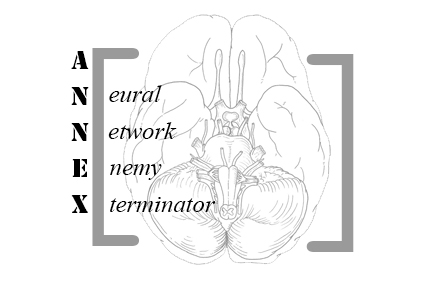
\includegraphics[width=0.75\textwidth]{logo}}

\rhead{Group \#2}

\lhead{CP468 Fall 2016}


\rfoot{Page \thepage}


\author{
  Morouney, Robert\\
  \href{mailto:robert@morouney.com}{robert@morouney.com}\texttt{ 069001422 }
   \and
   Rusu, David\\
   \href{mailto:davidrusu.me@gmail.com}{davidrusu.me@gmail.com}\texttt{ 131920260 }
}

%TODO: ADD DATE
\date{December 05 2016}

\begin{document}
  \maketitle
\begin{abstract}
Project Annex uses a recurrent neural net to learn the typing patterns of a user.  Using a system wide key logger, Annex attempts to dynamically track key strokes and constantly compare them to the patterns of the expected user.  Users keystroke patterns are determined by the summation of the dwell time and flight between consecutive key presses. Though this project came with many challenges in the end we were able to achieve an error rate of $~0.7\%$.
\end{abstract}
\tableofcontents
\chapter{Project Annex}
\epigraph{``We must annex those people. We can afflict them 
with our wise and beneficent government. We can introduce 
the novelty of thieves, all the way up from street-car 
pickpockets to municipal robbers and Government defaulters, 
and show them how amusing it is to arrest them and try them and 
then turn them loose''}{ \textit{Mark Twain}}
\section{A Brief Introduction to Authentication}
\paragraph{}User authentication is conventionally defined as a the comparisson between supplied user credentials and those stored in a trusted location such as a database. \cite{AUTH1} 
Though this model remains the standard it is far from perfect. 
The main issue with key based authentication is the user themselves. \cite{BADUSER}. 
This problem is lessened by methods such as two-factor authentication, finger-print and iris biometics but suffer from similar issues in users security.
In this report we focus on a less common biometirc method known as keystroke authentication \cite{BIOKEY1}.   

\paragraph{}For the past 3 years the ``Worldwide Threat Assessment of the US Intelligence Community'' \cite{US2014} \cite{US2015} \cite{US2016} has listed cyber threats as the top issue world security. 
Identity theft \cite{IDENT1}, Ransomware\cite{SRANS1} and bank fraud are a collective trillion dollar industry \cite{IDENT1}.  
Despite all of this users often choose passwords out of convinence rather than fear.  
In large password dumps the most common password is consistantly "12345678" and has been so for years. \cite{COMMONPASSWORD} 
To combat this system administrators have required users 
to frequently change passwords or choose password with increasing difficulty.  
\paragraph{}For this reason biometric authentication has been an active field of research.\cite{BIOMATIC} Most biometric identification techniques provide more entropy which in theory provides more security.
While it is unlikely an enemy could guess something as complex as a fingerprint, iris scan or DNA profile, once stolen, the victims identity would be compromised forever. \cite{IDTHEFT1}
\section{Meta Biometrics}
\paragraph{Keystroke Dynamics} studies the behaviorial pattern of individual users keystrokes based on timing of different events in a key press. \cite{KEYSTROKE1}
The two major timing events that define a key press are the \textit{Dwell Time} and the \textit{Flight Time} which are decribed in the figure below.
\begin{description}
\item[Dwell Time] time between key up and key down events.
\item[Flight Time] time between two key down events. 
\end{description}
\begin{center}
	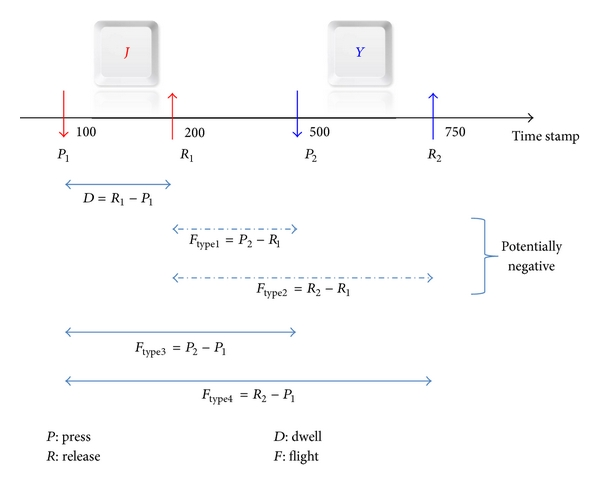
\includegraphics[width=.5\textwidth]{dwell_flight}
\end{center}
\paragraph{}By measuring the patterns of individual's Dwell and flight times for different key combinations a pattern can be determined which is able to identify that person with a certain degree of accuracy.
Over the past 20 years there have been many studies into the usage of keystorke dynamics as an authentication technique. \cite{KEYSTROKE2} \cite{KEYSTROKE3} \cite{KEYSTROKE4} \cite{KEYSTROKE5} \cite{KEYSTROKE6} 
\paragraph{}Improvments into machine learning and specifically studies of Neural Networks has vastly improved the accuracy of keystroke authentication techniques.   
Many of these studies have proven that the proper usage of keystroke dynamics can act as a reliable authentication technique \cite{KEYSTROKE7} and this has resulted in the release of some noteable consumer products. \cite{PROD1} \cite{PROD2} \cite{PROD3}

\chapter{Continuous Authentication}
\epigraph{``If you want to keep a secret, you must also hide it from yourself''}{ \textit{Geroge Orwell}}
\section{Our Approach}
\paragraph{}We aim to add to the many other studies in keystroke dynamics by providing a slightly different approach to authentication.
By continously logging a users keystrokes we can feed them into a recurrent neural network (RNN) in the form of a summation of the dwell and flight times between each key press event.
After training with only 100,000 key events our RNN was able to detect the user it was trained on within a 0.7\% accuracy. 

\begin{center}
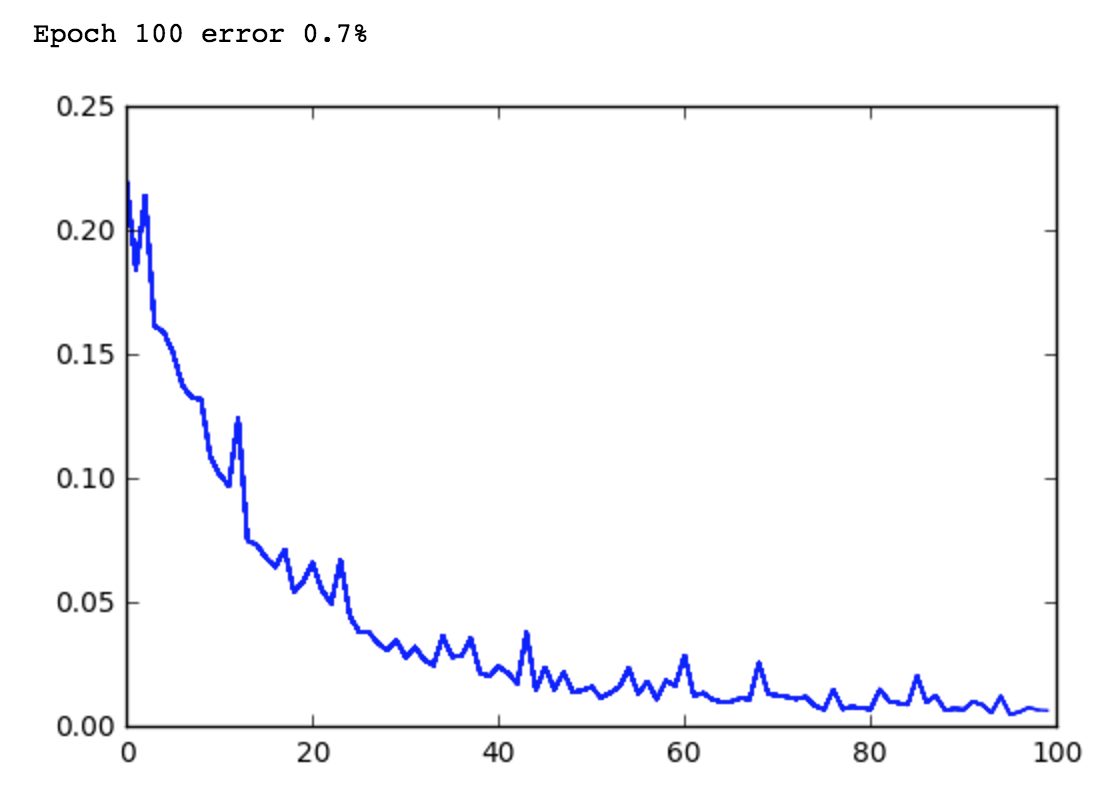
\includegraphics[width=0.5\textwidth]{graph1}
\end{center}

\paragraph{}Initially ANNEX must be trained with the desired users trusted keystrokes.  This can be accomplised over a few logged typinging sessions. 
Once the RNN is trained to the desired accuracy the program is put into monitoring mode where it decideds every 50 keystrokes if the user typing matches that of the accepted user.
\begin{center}
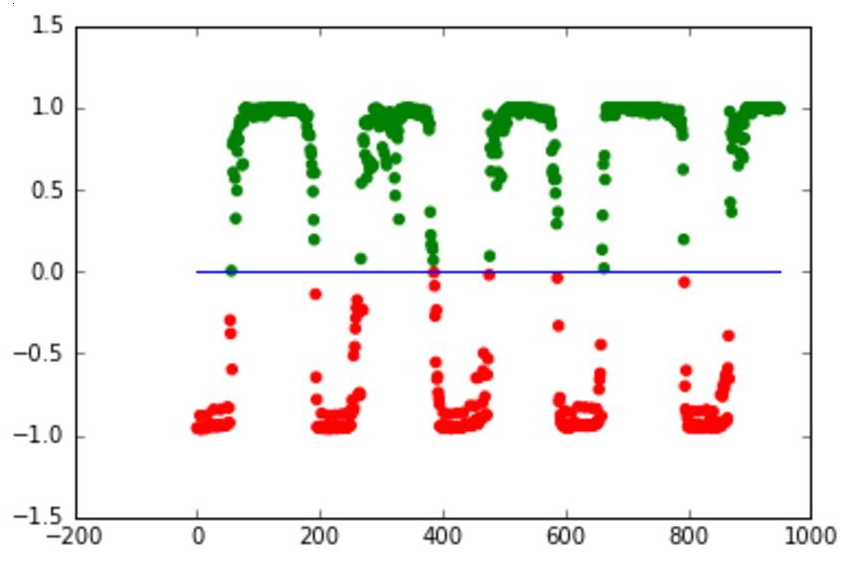
\includegraphics[width=0.5\textwidth]{graph2}
\end{center}
If a user is determined to be an intruder the program automatically sends a text message to a preprogrammed number and logs the event.
Since events, negative and positive, are constantly logged they can be  authenticated by the system administrator then used as training data to constantly improve the RNN. 
This allows the network to adapt to users changing typing styles over time and continuously maintain an acceptable accuracy.

\chapter{The RNN}
\section{The Recurrent Neural Network}
\paragraph{}ANNEX is built on top of tensorflow recurrent neural netork.  Each keyevent is inputted through the network with 3 normalized values.
The three inputs are the first key pressed, the second key pressed and the summation of the dwell time and flight time between the 2 press events. 
Each input is normalized to a range of $0.0000000$ to $1.0000000$. 
This was done through a process called unity based normalization where a known range can be reduced to [0,1] using the following formula:
$$X' = \frac{X - X_{min}}{X_{max}-X_{min}}$$
\paragraph{}The RNN itself is composed of 3 inputs with 32 hidden layers and 2 outputs.  The outputs represent the confidence levels of it not being the trained user and that of it being the correct user.  These confidence levels are used in conjuction to determine the likelyhood a user is authentic. 
The RNN then takes multiple samples until a confidence threshhold is reached and a decision can be made.
\begin{center}
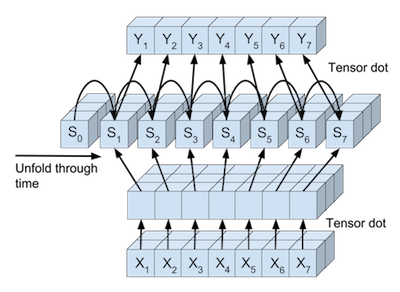
\includegraphics[width=0.25\textwidth]{RNN}
\end{center}
\chapter{The Code}
\section{Loading and normalizing the keystroke data}
\begin{lstlisting}[language=Python]
MAX_CHAR = 255
MIN_CHAR = 0

MIN_TIME = 10
MAX_TIME = 5000


def gaus_norm(x, MIN, MAX):
    return (float(x - MIN)/float(MAX-MIN))

def load_keystrokes(log_file):
    time_error_count = 0
    with open(log_file, 'r') as f:
        data = []
        last_char = None
        for line in f:
            time, char = [int(i) for i in line.split(',')]
            if last_char is None:
                last_char = char
                continue
            if time > MAX_TIME or time < MIN_TIME:
                time_error_count += 1
                continue
            
            new_time = gaus_norm(time, MIN_TIME, MAX_TIME)
            new_char = gaus_norm(char, MIN_CHAR, MAX_CHAR)
            new_last_char = gaus_norm(last_char, MIN_CHAR, MAX_CHAR)
            data.append([new_last_char, new_time, new_char])
            last_char = char

    data_count = len(data)

    print("Loaded {} events, {} time errors removed".format(data_count, time_error_count))
    return data

negative_data = load_keystrokes("key_logging/keystroke.log")
\end{lstliting}

\section{Set Up The RNN}
\begin{lstlisting}[language=Python]
# muddle positive time_delta data to generate negative samples
NUM_EXAMPLES = 100
SEQ_LENGTH = 200

assert all(len(data) >= SEQ_LENGTH for data in [david_data, robert_data, marcel_data]), 'need at least SEQ_LENGTH events'

def random_sub_seq(xs):
    # TODO extend to support variable size sequences
    start = int(np.random.uniform(0, len(xs) - SEQ_LENGTH))
    end = start + SEQ_LENGTH
    return xs[start:end]

train_input = []
train_output = []

for i in range(NUM_EXAMPLES * 10):
    if np.random.rand() < 0.5:
        # positive sample
        train_input.append(random_sub_seq(david_data))
        train_output.append([1, 0])
    else:
        # negative sample
        train_input.append(random_sub_seq(marcel_data))
        train_output.append([0, 1])

test_input = train_input[NUM_EXAMPLES:]
test_output = train_output[NUM_EXAMPLES:]
train_input = train_input[:NUM_EXAMPLES]
train_output = train_output[:NUM_EXAMPLES]

print("test and training data loaded")
data = tf.placeholder(tf.float32, [None, SEQ_LENGTH,2]) #Number of examples, number of input, dimension of each input
target = tf.placeholder(tf.float32, [None, 2])
num_hidden = 24
cell = tf.nn.rnn_cell.LSTMCell(num_hidden,state_is_tuple=True)
val, _ = tf.nn.dynamic_rnn(cell, data, dtype=tf.float32)
val = tf.transpose(val, [1, 0, 2])
last = tf.gather(val, int(val.get_shape()[0]) - 1)
weight = tf.Variable(tf.truncated_normal([num_hidden, int(target.get_shape()[1])]))
bias = tf.Variable(tf.constant(0.1, shape=[target.get_shape()[1]]))
prediction = tf.nn.softmax(tf.matmul(last, weight) + bias)
cross_entropy = -tf.reduce_sum(target * tf.log(prediction))
optimizer = tf.train.AdamOptimizer()
minimize = optimizer.minimize(cross_entropy)
mistakes = tf.not_equal(tf.argmax(target, 1), tf.argmax(prediction, 1))
error = tf.reduce_mean(tf.cast(mistakes, tf.float32))
\end{lstlisting}


\section{Train the RNN}


\begin{lstlisting}[language=Python]
batch_size = 10
no_of_batches = int(len(train_input)) // batch_size
epoch = 100
print("Batch size: {} || batches: {} || epochs: {}".format(batch_size, no_of_batches, epoch))

error_per_epoch = []

for i in range(epoch):
    ptr = 0
    for j in range(no_of_batches):
        inp, out = train_input[ptr:ptr+batch_size], train_output[ptr:ptr+batch_size]
        ptr+=batch_size
        sess.run(minimize,{data: inp, target: out})
    
 
    if i % 1 == 0:
        incorrect = sess.run(error,{data: test_input, target: test_output})
        error_per_epoch.append(incorrect)
        plt.plot(error_per_epoch, color='b')
        display.clear_output(wait=True)
        display.display(plt.gcf())
    
    # --- comment this out if you don't want to overwrite existing model
    save_path = saver.save(sess, "model.ckpt")

incorrect = sess.run(error,{data: test_input, target: test_output})
print('Epoch {:2d} error {:3.1f}\%'.format(i + 1, 100 * incorrect))

\end{lstlisting}

\section{Dynamic Authentication}
\begin{lstlisting}[language=Python]
current_keystrokes = load_keystrokes('./key_logging/keystroke.log')[-SEQ_LENGTH:]

inp, out = [current_keystrokes], [[1,0]]
result = sess.run(prediction,{data: inp}).mean(axis=0)
if result[0] > result[1]:
    print("Owner with {:.2f}% confidence".format(result[0] * 100))
else:    
    print("Intruder with {:.2f}% confidence".format(result[1] * 100))
print(result)

 --- can retrain model with this data --- 
sess.run(minimize,{data: inp, target: out})
print(sess.run(prediction,{data: [current_keystrokes]}).mean(axis=0))
\end{lstlisting}

\end{document}


%%%%%%%%%%%%%%%%%%%%%%%%%%%%%%%%%%%%%%%%%%%%%%%%%%%%%%%%%%%%%%%%%%%%%%%%%%%%%%%
% HELPFUL CODE:

% CODE SECTION
    %\code [language=C, caption=" "]
    %  %TODO: ADD CODE
    %\edoc

% PICTURE
    %\begin{center}
    %  \includegraphics[width=\textwidth]{diag} 
    %\end{center}

% GRAPH
    %\begin{tikzpicture}
    %  \begin{axis}[
    %    axis x line=middle,
    %    axis y line=middle,
    %    axis equal,
    %    xlabel = { }, %TODO ADD LABEL
    %    ylabel = { }, %TODO ADD LABEL
    %    restrict x to domain = -10:10, %TODO: ADD DOMAIN
    %    restrict y to domain = -10:10  %TODO: ADD DOMAIN
    %  ]
    %    \addplot[
    %      domain = -10:10, %TODO: CHANGE DOMAIN
    %      samples = 300
    %    ]{
    %      %TODO: ADD EQUATION
    %    }
    %  \end{axis}
    %\end{tikzpicture}

%SOME MATH
    % $ INLINE MATHS $
    % $$ SINGLE LINE MATH $$
    % MULTI LINE MATH:
      %\begin{align*}
      %  \left\{\:&\\
      %  &\vec{v} &= \vs1&2\\3&4\ve + \frac{3x^2+21}{-y_0^2+y_1^2*33.001} \\
      %  &&\textrm{where} \\
      %  &&\vec{y}\in\R \\
      %  \right\}
      %\end{align*}


